\documentclass{article}
\usepackage{amsmath}
\usepackage{amssymb}
\usepackage{graphicx}
\usepackage{hyperref}
\begin{document}

\providecommand{\pr}[1]{\ensuremath{\Pr\left(#1\right)}}
\providecommand{\prt}[2]{\ensuremath{p_{#1}^{\left(#2\right)} }}        % own macro for this question
\providecommand{\qfunc}[1]{\ensuremath{Q\left(#1\right)}}
\providecommand{\sbrak}[1]{\ensuremath{{}\left[#1\right]}}
\providecommand{\lsbrak}[1]{\ensuremath{{}\left[#1\right.}}
\providecommand{\rsbrak}[1]{\ensuremath{{}\left.#1\right]}}
\providecommand{\brak}[1]{\ensuremath{\left(#1\right)}}
\providecommand{\lbrak}[1]{\ensuremath{\left(#1\right.}}
\providecommand{\rbrak}[1]{\ensuremath{\left.#1\right)}}
\providecommand{\cbrak}[1]{\ensuremath{\left\{#1\right\}}}
\providecommand{\lcbrak}[1]{\ensuremath{\left\{#1\right.}}
\providecommand{\rcbrak}[1]{\ensuremath{\left.#1\right\}}}
\newcommand{\sgn}{\mathop{\mathrm{sgn}}}
\providecommand{\abs}[1]{\left\vert#1\right\vert}
\providecommand{\res}[1]{\Res\displaylimits_{#1}} 
\providecommand{\norm}[1]{\left\lVert#1\right\rVert}
%\providecommand{\norm}[1]{\lVert#1\rVert}
\providecommand{\mtx}[1]{\mathbf{#1}}
\providecommand{\mean}[1]{E\left[ #1 \right]}
\providecommand{\cond}[2]{#1\middle|#2}
\providecommand{\fourier}{\overset{\mathcal{F}}{ \rightleftharpoons}}
\newenvironment{amatrix}[1]{%
  \left(\begin{array}{@{}*{#1}{c}|c@{}}
}{%
  \end{array}\right)
}
%\providecommand{\hilbert}{\overset{\mathcal{H}}{ \rightleftharpoons}}
%\providecommand{\system}{\overset{\mathcal{H}}{ \longleftrightarrow}}
	%\newcommand{\solution}[2]{\textbf{Solution:}{#1}}
\newcommand{\solution}{\noindent \textbf{Solution: }}
\newcommand{\cosec}{\,\text{cosec}\,}
\providecommand{\dec}[2]{\ensuremath{\overset{#1}{\underset{#2}{\gtrless}}}}
\newcommand{\myvec}[1]{\ensuremath{\begin{pmatrix}#1\end{pmatrix}}}
\newcommand{\mydet}[1]{\ensuremath{\begin{vmatrix}#1\end{vmatrix}}}
\newcommand{\myaugvec}[2]{\ensuremath{\begin{amatrix}{#1}#2\end{amatrix}}}
\providecommand{\rank}{\text{rank}}
\providecommand{\pr}[1]{\ensuremath{\Pr\left(#1\right)}}
\providecommand{\qfunc}[1]{\ensuremath{Q\left(#1\right)}}
	\newcommand*{\permcomb}[4][0mu]{{{}^{#3}\mkern#1#2_{#4}}}
\newcommand*{\perm}[1][-3mu]{\permcomb[#1]{P}}
\newcommand*{\comb}[1][-1mu]{\permcomb[#1]{C}}
\providecommand{\qfunc}[1]{\ensuremath{Q\left(#1\right)}}
\providecommand{\gauss}[2]{\mathcal{N}\ensuremath{\left(#1,#2\right)}}
\providecommand{\diff}[2]{\ensuremath{\frac{d{#1}}{d{#2}}}}
\providecommand{\myceil}[1]{\left \lceil #1 \right \rceil }
\newcommand\figref{Fig.~\ref}
\newcommand\tabref{Table~\ref}
\newcommand{\sinc}{\,\text{sinc}\,}
\newcommand{\rect}{\,\text{rect}\,}
%%
%	%\newcommand{\solution}[2]{\textbf{Solution:}{#1}}
%\newcommand{\solution}{\noindent \textbf{Solution: }}
%\newcommand{\cosec}{\,\text{cosec}\,}
%\numberwithin{equation}{section}
%\numberwithin{equation}{subsection}
%\numberwithin{problem}{section}
%\numberwithin{definition}{section}
%\makeatletter
%\@addtoreset{figure}{problem}
%\makeatother

%\let\StandardTheFigure\thefigure
\let\vec\mathbf
Suppose the equations $AB, BC$ and $CA$ are respectively given by 
                 %niTx = ci i = 1,2,3                 (1.5.1.1)
                 \begin{align}
                 \label{eq:a}
                 \vec{n_i}^{\top}\vec{x} &= c_i
                 \end{align}      
                \[i=1,2,3\]
The equations of the respective angle bisectors are then given by
                % (niTx-ci)/||ni|| = +- (njTx-cj)/||nj|| i=/j              (1.5.1.2)
\begin{align}
\label{eq:b}
\frac{\vec{n_i}^{\top}\vec{x}-c_i}{\norm{\vec{n_i}}} &= \pm\frac{\vec{n_j}^{\top}\vec{x}-c_j}{\norm{{\vec{n_j}}}}
\end{align}
\[i \neq j\]
Substitute numerical values and find the equations of the angle bisectors of $\vec{A},\vec{B}$ and $\vec{C}$.

\solution:
   
Given $\vec{A} = \myvec{1\\-1}, \vec{B} = \myvec{-4\\6}$ and $\vec{C} = \myvec{-3\\-5}$
 \\The normal form of a line is 
           %nT(x-A) = 0   where n = (0 1  m  and m = B - A
                                    
           \begin{align}
           \label{eq:c}
           \vec{n}^{\top}(\vec{x}-\vec{A}) &= 0   
           \end{align}
           where $\vec{n} = \myvec{0&1\\-1&1}\vec{m}$ and $\vec{m} = (\vec{B} - \vec{A})$, where $\vec{A}$, $\vec{B}$ are two points on the line and $\vec{m}$ is slope vector of the line.\\
 From solution 1.1.5,
         \begin{align}
         \label{eq:e}
        AB : \myvec{7&5}\vec{x} &= 2
        \end{align}
                 \begin{align}
          \label{eq:f}
         BC : \myvec{-11&-1}\vec{x} &= -10
        \end{align}
        \begin{align}
  \label{eq:d}
        CA : \myvec{4&-4}\vec{x} &= 8
        \end{align}
            
By comparing eq.\ref{eq:a}, eq.\ref{eq:e},  eq.\ref{eq:f},  eq.\ref{eq:d}  :
     
     \[\vec{n_1} = \myvec{7\\5}\] 
    \[ \vec{n_2} = \myvec{-11\\-1} \]   
  \[ \vec{n_3} = \myvec{4\\-4} \]
  
            and
   
    \[c_1 = 2\] 
 \[  c_2 = -10 \]
   \[c_3 = 8   \]
     
            
     From eq \ref{eq:b}, the equation of internal angle bisector is  : 
                 \begin{align}\frac{\vec{n_i}^{\top}\vec{x}-c_i}{\norm{\vec{n_i}}} &= \frac{\vec{n_j}^{\top}\vec{x}-c_j}{\norm{{\vec{n_j}}}} 
                 \end{align}
  $\implies$ Internal angle bisector of $\vec{B}$ (i=1 , j=2) : 
                  \begin{align}  \frac{\myvec{7&5}\vec{x}-2}{\norm{\myvec{7\\5}}} &=\frac{\myvec{-11&-1}\vec{x}-10}{\norm{{\myvec{-11\\-1}}}}
                  \end{align}
 \begin{align}\because  \norm{\myvec{x_1\\x_2}} &= \sqrt{x_1^2+x_2^2} 
 \end{align}  :
      
  \begin{align} \implies    \frac{\myvec{7&5}\vec{x}-2}{\sqrt{74}} &=\frac{\myvec{11&-1}\vec{x}-10}{\sqrt{122}}
  \end{align}                                
   \begin{align} \implies    \frac{\myvec{7&5}\vec{x}-2}{\sqrt{37}} &=\frac{\myvec{11&-1}\vec{x}-10}{\sqrt{61}}
   \end{align} 
    $\therefore$ Internal angle bisector of $\vec{B}$ :                                                          
\begin{align}    \myvec{7\sqrt{61}-11\sqrt{37}&5\sqrt{61}+\sqrt{37}}\vec{x} &=2(\sqrt{61}-5\sqrt{37})
\end{align}   
                           \[or\]
     \begin{align}\myvec{-12.2386&45.1304}\vec{x} &=-45.2071 
     \end{align}                         
     

\begin{figure}[htbp]
\centerline{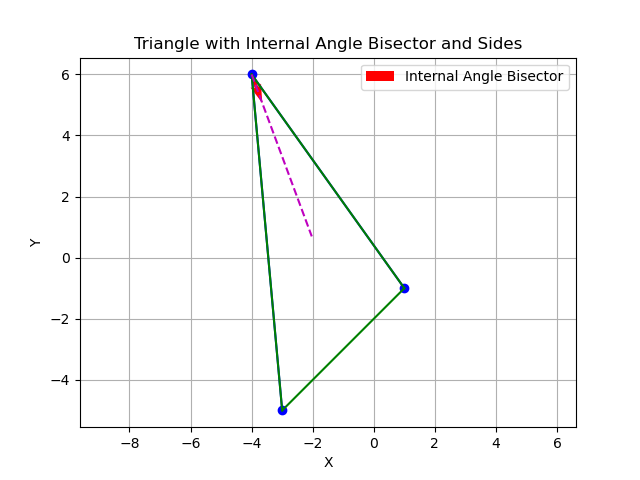
\includegraphics{Figure_1.png}}
\caption{Angle bisector of $\vec{B}$.}
\label{fig}
\end{figure}
\end{document}


